\PassOptionsToPackage{unicode=true}{hyperref} % options for packages loaded elsewhere
\PassOptionsToPackage{hyphens}{url}
%
\documentclass[]{article}
\usepackage{lmodern}
\usepackage{amssymb,amsmath}
\usepackage{ifxetex,ifluatex}
\usepackage{fixltx2e} % provides \textsubscript
\ifnum 0\ifxetex 1\fi\ifluatex 1\fi=0 % if pdftex
  \usepackage[T1]{fontenc}
  \usepackage[utf8]{inputenc}
  \usepackage{textcomp} % provides euro and other symbols
\else % if luatex or xelatex
  \usepackage{unicode-math}
  \defaultfontfeatures{Ligatures=TeX,Scale=MatchLowercase}
\fi
% use upquote if available, for straight quotes in verbatim environments
\IfFileExists{upquote.sty}{\usepackage{upquote}}{}
% use microtype if available
\IfFileExists{microtype.sty}{%
\usepackage[]{microtype}
\UseMicrotypeSet[protrusion]{basicmath} % disable protrusion for tt fonts
}{}
\IfFileExists{parskip.sty}{%
\usepackage{parskip}
}{% else
\setlength{\parindent}{0pt}
\setlength{\parskip}{6pt plus 2pt minus 1pt}
}
\usepackage{hyperref}
\hypersetup{
            pdftitle={Re-analysis of Marin-Carli et al sMEC Data},
            pdfauthor={Dave Bridges},
            pdfborder={0 0 0},
            breaklinks=true}
\urlstyle{same}  % don't use monospace font for urls
\usepackage[margin=1in]{geometry}
\usepackage{color}
\usepackage{fancyvrb}
\newcommand{\VerbBar}{|}
\newcommand{\VERB}{\Verb[commandchars=\\\{\}]}
\DefineVerbatimEnvironment{Highlighting}{Verbatim}{commandchars=\\\{\}}
% Add ',fontsize=\small' for more characters per line
\usepackage{framed}
\definecolor{shadecolor}{RGB}{248,248,248}
\newenvironment{Shaded}{\begin{snugshade}}{\end{snugshade}}
\newcommand{\AlertTok}[1]{\textcolor[rgb]{0.94,0.16,0.16}{#1}}
\newcommand{\AnnotationTok}[1]{\textcolor[rgb]{0.56,0.35,0.01}{\textbf{\textit{#1}}}}
\newcommand{\AttributeTok}[1]{\textcolor[rgb]{0.77,0.63,0.00}{#1}}
\newcommand{\BaseNTok}[1]{\textcolor[rgb]{0.00,0.00,0.81}{#1}}
\newcommand{\BuiltInTok}[1]{#1}
\newcommand{\CharTok}[1]{\textcolor[rgb]{0.31,0.60,0.02}{#1}}
\newcommand{\CommentTok}[1]{\textcolor[rgb]{0.56,0.35,0.01}{\textit{#1}}}
\newcommand{\CommentVarTok}[1]{\textcolor[rgb]{0.56,0.35,0.01}{\textbf{\textit{#1}}}}
\newcommand{\ConstantTok}[1]{\textcolor[rgb]{0.00,0.00,0.00}{#1}}
\newcommand{\ControlFlowTok}[1]{\textcolor[rgb]{0.13,0.29,0.53}{\textbf{#1}}}
\newcommand{\DataTypeTok}[1]{\textcolor[rgb]{0.13,0.29,0.53}{#1}}
\newcommand{\DecValTok}[1]{\textcolor[rgb]{0.00,0.00,0.81}{#1}}
\newcommand{\DocumentationTok}[1]{\textcolor[rgb]{0.56,0.35,0.01}{\textbf{\textit{#1}}}}
\newcommand{\ErrorTok}[1]{\textcolor[rgb]{0.64,0.00,0.00}{\textbf{#1}}}
\newcommand{\ExtensionTok}[1]{#1}
\newcommand{\FloatTok}[1]{\textcolor[rgb]{0.00,0.00,0.81}{#1}}
\newcommand{\FunctionTok}[1]{\textcolor[rgb]{0.00,0.00,0.00}{#1}}
\newcommand{\ImportTok}[1]{#1}
\newcommand{\InformationTok}[1]{\textcolor[rgb]{0.56,0.35,0.01}{\textbf{\textit{#1}}}}
\newcommand{\KeywordTok}[1]{\textcolor[rgb]{0.13,0.29,0.53}{\textbf{#1}}}
\newcommand{\NormalTok}[1]{#1}
\newcommand{\OperatorTok}[1]{\textcolor[rgb]{0.81,0.36,0.00}{\textbf{#1}}}
\newcommand{\OtherTok}[1]{\textcolor[rgb]{0.56,0.35,0.01}{#1}}
\newcommand{\PreprocessorTok}[1]{\textcolor[rgb]{0.56,0.35,0.01}{\textit{#1}}}
\newcommand{\RegionMarkerTok}[1]{#1}
\newcommand{\SpecialCharTok}[1]{\textcolor[rgb]{0.00,0.00,0.00}{#1}}
\newcommand{\SpecialStringTok}[1]{\textcolor[rgb]{0.31,0.60,0.02}{#1}}
\newcommand{\StringTok}[1]{\textcolor[rgb]{0.31,0.60,0.02}{#1}}
\newcommand{\VariableTok}[1]{\textcolor[rgb]{0.00,0.00,0.00}{#1}}
\newcommand{\VerbatimStringTok}[1]{\textcolor[rgb]{0.31,0.60,0.02}{#1}}
\newcommand{\WarningTok}[1]{\textcolor[rgb]{0.56,0.35,0.01}{\textbf{\textit{#1}}}}
\usepackage{longtable,booktabs}
% Fix footnotes in tables (requires footnote package)
\IfFileExists{footnote.sty}{\usepackage{footnote}\makesavenoteenv{longtable}}{}
\usepackage{graphicx,grffile}
\makeatletter
\def\maxwidth{\ifdim\Gin@nat@width>\linewidth\linewidth\else\Gin@nat@width\fi}
\def\maxheight{\ifdim\Gin@nat@height>\textheight\textheight\else\Gin@nat@height\fi}
\makeatother
% Scale images if necessary, so that they will not overflow the page
% margins by default, and it is still possible to overwrite the defaults
% using explicit options in \includegraphics[width, height, ...]{}
\setkeys{Gin}{width=\maxwidth,height=\maxheight,keepaspectratio}
\setlength{\emergencystretch}{3em}  % prevent overfull lines
\providecommand{\tightlist}{%
  \setlength{\itemsep}{0pt}\setlength{\parskip}{0pt}}
\setcounter{secnumdepth}{5}
% Redefines (sub)paragraphs to behave more like sections
\ifx\paragraph\undefined\else
\let\oldparagraph\paragraph
\renewcommand{\paragraph}[1]{\oldparagraph{#1}\mbox{}}
\fi
\ifx\subparagraph\undefined\else
\let\oldsubparagraph\subparagraph
\renewcommand{\subparagraph}[1]{\oldsubparagraph{#1}\mbox{}}
\fi

% set default figure placement to htbp
\makeatletter
\def\fps@figure{htbp}
\makeatother


\title{Re-analysis of Marin-Carli et al sMEC Data}
\author{Dave Bridges}
\date{January 4, 2021}

\begin{document}
\maketitle

{
\setcounter{tocdepth}{2}
\tableofcontents
}
\hypertarget{purpose}{%
\section{Purpose}\label{purpose}}

To re-analyse cell populations from the Martin-Carli \emph{et al}'s
scRNAseq study of lactating mammary glands. This work is described in
Martin Carli et al. (2020). This follows the analysis flow suggested for
Seurat 3.2 seen at
\url{https://satijalab.org/seurat/v3.2/pbmc3k_tutorial.html}

\hypertarget{data-input}{%
\section{Data Input}\label{data-input}}

Downloaded the data from GSE15889 and removed prefixes from filenames.

\hypertarget{preprocessing}{%
\subsection{Preprocessing}\label{preprocessing}}

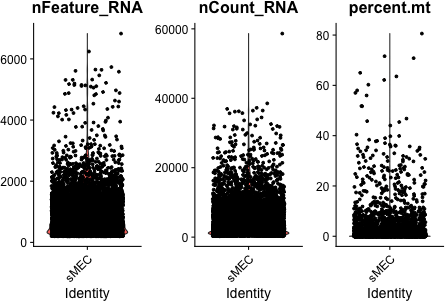
\includegraphics{figures/pre-processing-1.png}
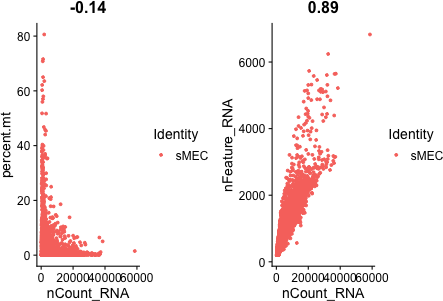
\includegraphics{figures/pre-processing-2.png} \#\# Normalizing Data

Normalizes the feature expression for each cell by the total expression
x 1000, then log transforms

\hypertarget{highly-variable-features}{%
\subsection{Highly Variable Features}\label{highly-variable-features}}

Features with high cell to cell variability (highly expressed in some
cells but not others)

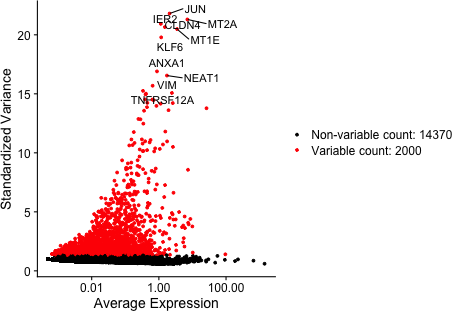
\includegraphics{figures/variable-features-1.png}

\hypertarget{scaling}{%
\subsection{Scaling}\label{scaling}}

Shifts expression so that mean expression across cells is 0, and
variance is 1. This reduces the impact of outliers on downstream
analyses. We did not regress out specific sources of heterogeneity like
mitochondrial contamination or cell cycle stage.

\hypertarget{dimensionality-reductions}{%
\section{Dimensionality Reductions}\label{dimensionality-reductions}}

\begin{verbatim}
## PC_ 1 
## Positive:  SPP1, CLU, SCGB3A1, HPGD, MYBPC1 
## Negative:  MALAT1, NEAT1, KLF6, JUNB, BTG1 
## PC_ 2 
## Positive:  CLDN4, TNFRSF12A, ELF3, MT1E, ATF3 
## Negative:  SRGN, PTPRC, LAPTM5, CD52, CXCR4 
## PC_ 3 
## Positive:  TYROBP, FCER1G, SPI1, CD68, FABP5 
## Negative:  ETS1, TRAC, CD3E, CD2, FYN 
## PC_ 4 
## Positive:  KIAA0101, TYMS, PTTG1, STMN1, CCNB1 
## Negative:  NEAT1, MT-CO3, MT-CO1, MT-ND4, XIST 
## PC_ 5 
## Positive:  S100A10, S100A6, FTL, S100A4, HCST 
## Negative:  KIAA0101, BIRC5, CCNB1, TYMS, TOP2A
\end{verbatim}

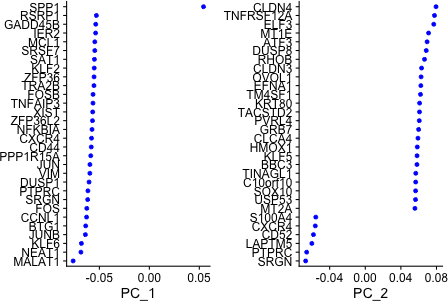
\includegraphics{figures/dimensionality-pca-1.png}
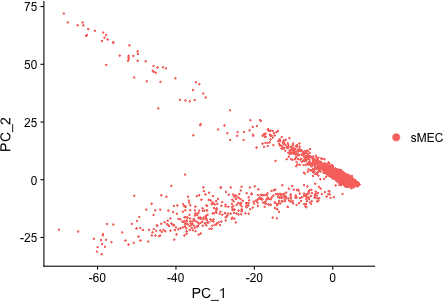
\includegraphics{figures/dimensionality-pca-2.png}
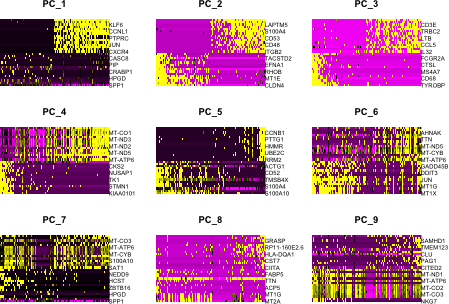
\includegraphics{figures/dimensionality-pca-3.png}

\hypertarget{determination-of-number-of-clusters}{%
\section{Determination of Number of
Clusters}\label{determination-of-number-of-clusters}}

Used the JackStraw procedure in Macosko et al. (2015), sampling 1\% of
the data re-running the PCA and constructing a null distribution of
feature scores, then repeating. This identified `significant' PCs. We
also did an elbow plot.

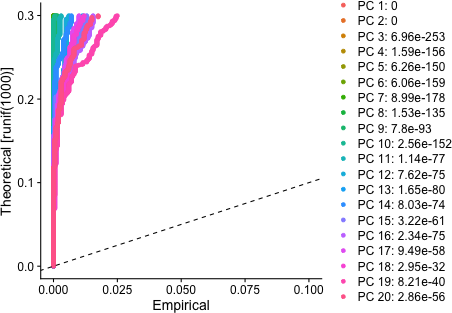
\includegraphics{figures/cluster-numbers-1.png}
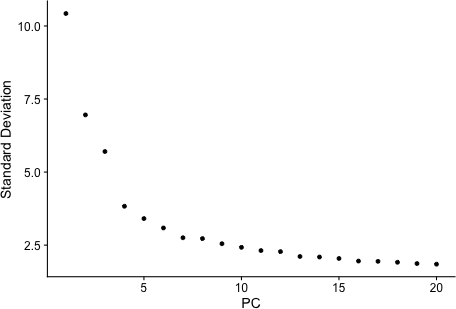
\includegraphics{figures/cluster-numbers-2.png}

Based on this we decided to use 13 PCs to cluster the cells.

\hypertarget{clustering-cell-types}{%
\section{Clustering Cell Types}\label{clustering-cell-types}}

Seurat 3.2 uses a K-nearest neighbor approach then tries to partition
this into commmunities of cell types.

\hypertarget{identification-and-assignment-of-clusters}{%
\subsection{Identification and Assignment of
Clusters}\label{identification-and-assignment-of-clusters}}

\begin{verbatim}
## Modularity Optimizer version 1.3.0 by Ludo Waltman and Nees Jan van Eck
## 
## Number of nodes: 5917
## Number of edges: 202546
## 
## Running Louvain algorithm...
## Maximum modularity in 10 random starts: 0.8391
## Number of communities: 9
## Elapsed time: 0 seconds
\end{verbatim}

\hypertarget{non-linear-dimensionality-reduction}{%
\subsection{Non-Linear Dimensionality
Reduction}\label{non-linear-dimensionality-reduction}}

Did both UMAP and t-SNE plots using 13 clusters

\hypertarget{umap}{%
\subsubsection{UMAP}\label{umap}}

\begin{figure}
\centering
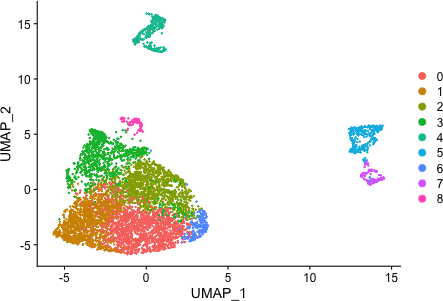
\includegraphics{figures/umap-plot-initial-1.png}
\caption{UMAP plot of secreted MECs}
\end{figure}

\hypertarget{t-sne-plots}{%
\subsubsection{t-SNE Plots}\label{t-sne-plots}}

\begin{figure}
\centering
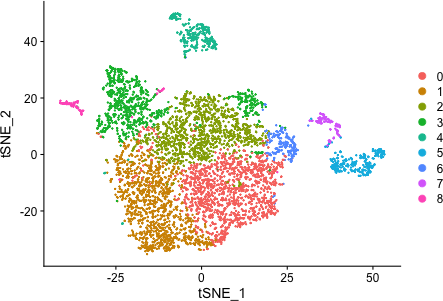
\includegraphics{figures/tsne-plot-initial-1.png}
\caption{t-SNE plot of secreted MECs}
\end{figure}

\begin{longtable}[]{@{}rrrrrll@{}}
\caption{Cell Specific Markers (All)}\tabularnewline
\toprule
p\_val & avg\_logFC & pct.1 & pct.2 & p\_val\_adj & cluster &
gene\tabularnewline
\midrule
\endfirsthead
\toprule
p\_val & avg\_logFC & pct.1 & pct.2 & p\_val\_adj & cluster &
gene\tabularnewline
\midrule
\endhead
0 & 0.773 & 0.635 & 0.077 & 0 & 2 & C4BPA\tabularnewline
0 & 0.510 & 0.595 & 0.055 & 0 & 2 & HLA-DRB5\tabularnewline
0 & 1.537 & 0.940 & 0.574 & 0 & 3 & CLU\tabularnewline
0 & 1.409 & 0.600 & 0.165 & 0 & 3 & KRT15\tabularnewline
0 & 4.451 & 0.675 & 0.042 & 0 & 4 & MT1E\tabularnewline
0 & 4.749 & 0.773 & 0.103 & 0 & 4 & MT2A\tabularnewline
0 & 3.261 & 0.997 & 0.136 & 0 & 5 & MALAT1\tabularnewline
0 & 2.832 & 0.994 & 0.545 & 0 & 5 & MT-ATP6\tabularnewline
0 & 1.743 & 1.000 & 0.666 & 0 & 6 & MT-CO1\tabularnewline
0 & 1.606 & 1.000 & 0.651 & 0 & 6 & MT-CO3\tabularnewline
0 & 3.163 & 0.852 & 0.422 & 0 & 7 & CD74\tabularnewline
0 & 3.184 & 0.911 & 0.834 & 0 & 7 & FTL\tabularnewline
0 & 1.985 & 0.717 & 0.083 & 0 & 8 & STMN1\tabularnewline
0 & 1.962 & 0.808 & 0.319 & 0 & 8 & H2AFZ\tabularnewline
\bottomrule
\end{longtable}

\hypertarget{feature-analysis}{%
\section{Feature Analysis}\label{feature-analysis}}

\hypertarget{analysis-of-clusters}{%
\subsection{Analysis of clusters}\label{analysis-of-clusters}}

\begin{longtable}[]{@{}lrrrrrll@{}}
\caption{Clusters of genes of interest}\tabularnewline
\toprule
& p\_val & avg\_logFC & pct.1 & pct.2 & p\_val\_adj & cluster &
gene\tabularnewline
\midrule
\endfirsthead
\toprule
& p\_val & avg\_logFC & pct.1 & pct.2 & p\_val\_adj & cluster &
gene\tabularnewline
\midrule
\endhead
CSN2 & 0 & 0.504 & 1.000 & 0.988 & 0.000 & 2 & CSN2\tabularnewline
FASN & 0 & 0.735 & 0.848 & 0.756 & 0.007 & 6 & FASN\tabularnewline
\bottomrule
\end{longtable}

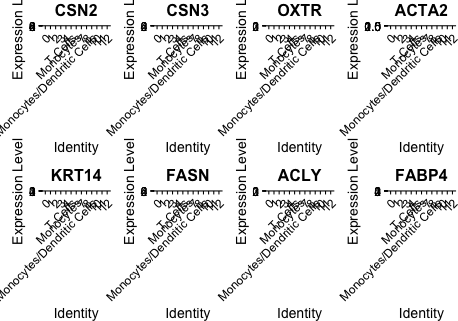
\includegraphics{figures/feature-analysis-1.png}
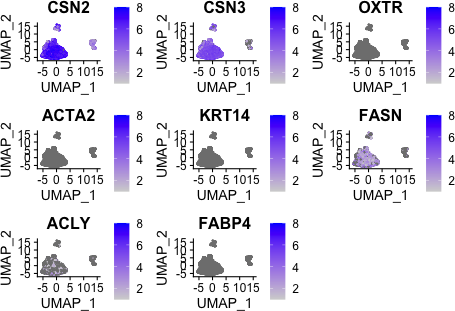
\includegraphics{figures/feature-analysis-2.png}
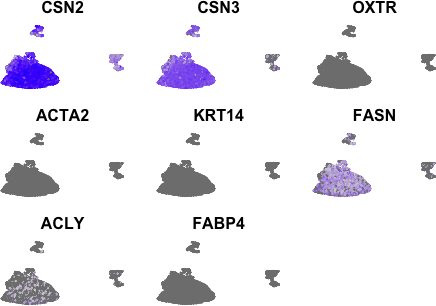
\includegraphics{figures/feature-analysis-3.png}
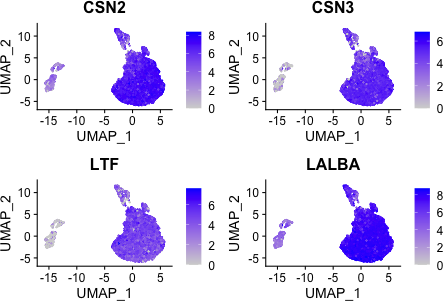
\includegraphics{figures/feature-analysis-4.png}
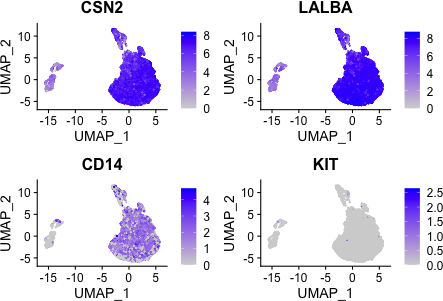
\includegraphics{figures/feature-analysis-5.png}
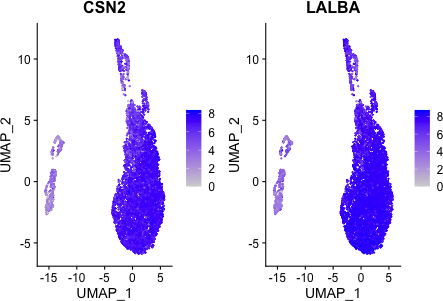
\includegraphics{figures/feature-analysis-6.png}
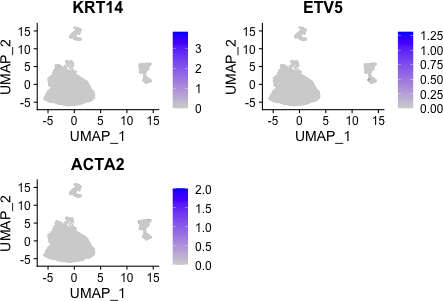
\includegraphics{figures/feature-analysis-7.png}
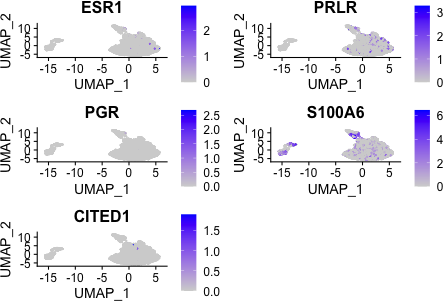
\includegraphics{figures/feature-analysis-8.png}
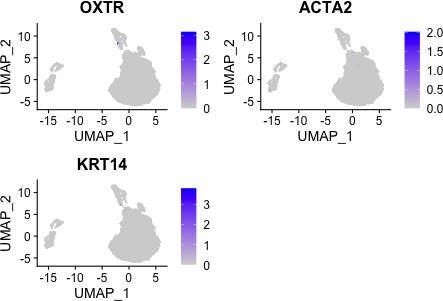
\includegraphics{figures/feature-analysis-9.png}
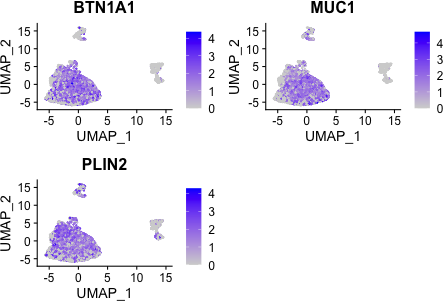
\includegraphics{figures/feature-analysis-10.png}
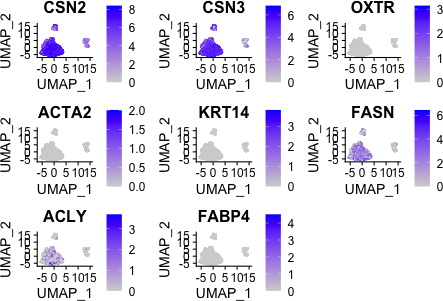
\includegraphics{figures/feature-analysis-11.png}
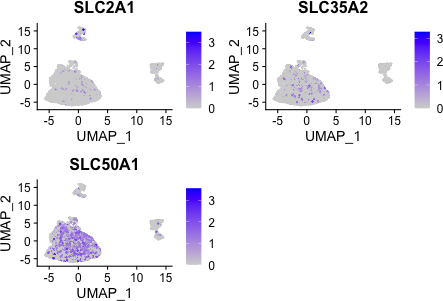
\includegraphics{figures/feature-analysis-12.png}
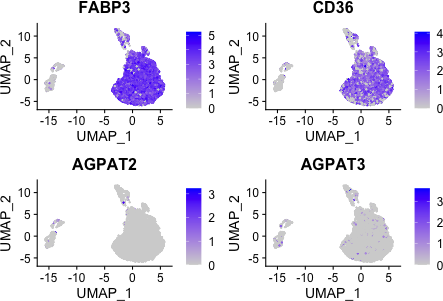
\includegraphics{figures/feature-analysis-13.png}
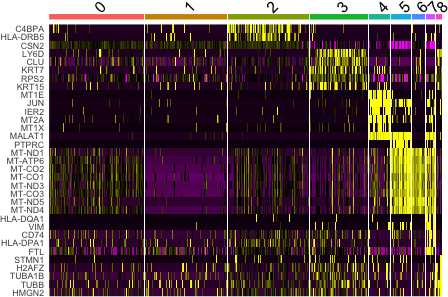
\includegraphics{figures/feature-analysis-14.png}

\hypertarget{session-information}{%
\section{Session Information}\label{session-information}}

\begin{Shaded}
\begin{Highlighting}[]
\KeywordTok{sessionInfo}\NormalTok{()}
\end{Highlighting}
\end{Shaded}

\begin{verbatim}
## R version 4.0.2 (2020-06-22)
## Platform: x86_64-apple-darwin17.0 (64-bit)
## Running under: macOS  10.16
## 
## Matrix products: default
## BLAS:   /Library/Frameworks/R.framework/Versions/4.0/Resources/lib/libRblas.dylib
## LAPACK: /Library/Frameworks/R.framework/Versions/4.0/Resources/lib/libRlapack.dylib
## 
## locale:
## [1] en_US.UTF-8/en_US.UTF-8/en_US.UTF-8/C/en_US.UTF-8/en_US.UTF-8
## 
## attached base packages:
## [1] stats     graphics  grDevices utils     datasets  methods   base     
## 
## other attached packages:
## [1] ggplot2_3.3.2 Seurat_3.2.3  dplyr_1.0.2   tidyr_1.1.2   knitr_1.30   
## 
## loaded via a namespace (and not attached):
##   [1] nlme_3.1-151          matrixStats_0.57.0    RcppAnnoy_0.0.18     
##   [4] RColorBrewer_1.1-2    httr_1.4.2            sctransform_0.3.2    
##   [7] tools_4.0.2           R6_2.5.0              irlba_2.3.3          
##  [10] rpart_4.1-15          KernSmooth_2.23-18    uwot_0.1.10          
##  [13] mgcv_1.8-33           lazyeval_0.2.2        colorspace_2.0-0     
##  [16] withr_2.3.0           tidyselect_1.1.0      gridExtra_2.3        
##  [19] compiler_4.0.2        plotly_4.9.2.2        labeling_0.4.2       
##  [22] scales_1.1.1          lmtest_0.9-38         spatstat.data_1.7-0  
##  [25] ggridges_0.5.2        pbapply_1.4-3         spatstat_1.64-1      
##  [28] goftest_1.2-2         stringr_1.4.0         digest_0.6.27        
##  [31] spatstat.utils_1.17-0 rmarkdown_2.6         pkgconfig_2.0.3      
##  [34] htmltools_0.5.0       parallelly_1.22.0     limma_3.44.3         
##  [37] highr_0.8             fastmap_1.0.1         htmlwidgets_1.5.3    
##  [40] rlang_0.4.10          shiny_1.5.0           farver_2.0.3         
##  [43] generics_0.1.0        zoo_1.8-8             jsonlite_1.7.2       
##  [46] ica_1.0-2             magrittr_2.0.1        patchwork_1.1.1      
##  [49] Matrix_1.2-18         Rcpp_1.0.5            munsell_0.5.0        
##  [52] abind_1.4-5           reticulate_1.18       lifecycle_0.2.0      
##  [55] stringi_1.5.3         yaml_2.2.1            MASS_7.3-53          
##  [58] Rtsne_0.15            plyr_1.8.6            grid_4.0.2           
##  [61] parallel_4.0.2        listenv_0.8.0         promises_1.1.1       
##  [64] ggrepel_0.9.0         crayon_1.3.4          deldir_0.2-3         
##  [67] miniUI_0.1.1.1        lattice_0.20-41       cowplot_1.1.0        
##  [70] splines_4.0.2         tensor_1.5            magick_2.5.2         
##  [73] pillar_1.4.7          igraph_1.2.6          future.apply_1.6.0   
##  [76] reshape2_1.4.4        codetools_0.2-18      leiden_0.3.6         
##  [79] glue_1.4.2            evaluate_0.14         data.table_1.13.4    
##  [82] vctrs_0.3.6           png_0.1-7             httpuv_1.5.4         
##  [85] gtable_0.3.0          RANN_2.6.1            purrr_0.3.4          
##  [88] polyclip_1.10-0       scattermore_0.7       future_1.21.0        
##  [91] xfun_0.19             rsvd_1.0.3            mime_0.9             
##  [94] xtable_1.8-4          RSpectra_0.16-0       later_1.1.0.1        
##  [97] survival_3.2-7        viridisLite_0.3.0     tibble_3.0.4         
## [100] cluster_2.1.0         globals_0.14.0        fitdistrplus_1.1-3   
## [103] ellipsis_0.3.1        ROCR_1.0-11
\end{verbatim}

\hypertarget{refs}{}
\leavevmode\hypertarget{ref-Macosko2015}{}%
Macosko, Evan Z., Anindita Basu, Rahul Satija, James Nemesh, Karthik
Shekhar, Melissa Goldman, Itay Tirosh, et al. 2015. ``Highly parallel
genome-wide expression profiling of individual cells using nanoliter
droplets.'' \emph{Cell} 161 (5). Elsevier: 1202--14.
\url{https://doi.org/10.1016/j.cell.2015.05.002}.

\leavevmode\hypertarget{ref-MartinCarli2020}{}%
Martin Carli, Jayne F., G. Devon Trahan, Kenneth L. Jones, Nicole
Hirsch, Kristy P. Rolloff, Emily Z. Dunn, Jacob E. Friedman, et al.
2020. ``Single Cell RNA Sequencing of Human Milk-Derived Cells Reveals
Sub-Populations of Mammary Epithelial Cells with Molecular Signatures of
Progenitor and Mature States: a Novel, Non-invasive Framework for
Investigating Human Lactation Physiology.'' \emph{Journal of Mammary
Gland Biology and Neoplasia}. Journal of Mammary Gland Biology;
Neoplasia. \url{https://doi.org/10.1007/s10911-020-09466-z}.

\end{document}
